

\subsection{Jazyky}
\indent
Strucny popis jazyka a veci s nim spojenych. 


  
\section{Anal�za jazykov}
\indent 
https://w3techs.com/technologies/comparison/os-linux,os-windows
\newline
Pod?a tejto str�nky linux pou��va 36.9\% a Windows 33.3\% serverov.
Najpou????van???m jazykom pre linuxov??? verziu os je shell, pre Windows je to powershell.
Avsak v dnesnej dobe existuje velke mnozstvo skriptovacich jazykov, ktore ponukaju podobnu funkcionalitu ako vyssie spominane.

\subsection{Priprava analyzy existujucich }
vyber skriptovacich jazykov pre analyzua - sh, bat, lua, py, js, coffe
vytvorenie shell scriptu, ktory analyzuje data
- zamerali sme sa na hladanie klucovych slov v zdrojovych suboroch roznych open source projektoch, ich zoznam pripajame v prilohach
- podla vyskytu jednotlivych klucovych slov sme 

\section{Jazyky}
Pri programovac�ch jazykoch n�s zauj�maj� ich vyjadrovacie schopnosti ako aj vlastnosti z h�adiska ich rozpoznania.
Tieto vlastnosti sa t�kaj� programovania a prekladu, pri�om obe je potrebn� zoh�adni� pri tvorbe jazyka.
V dne�nej dobe sa pou��vaj� na programovanie hlavne takzvan� vy��ie programovacie jazyky, m��eme ich ozna�i� ako zdrojov� jazyky.
Na to aby vykon�vali �o pou��vate� naprogramoval je potrebn� aby pretransformova� ich do jazyka dam�ho stroja.
Spom�nan� transform�ciu zabezpe�uje preklada�, preklada�om m�me na mysli program, ktor� ��ta zdrojov� jazyk a transformuje ho do
cie�ov�ho jazyka, ktor�mu rozumie stroj.

\subsection{Proces prekladu}
Aby bol preklad mo�n�, mus� by� zdrojov� k�d programu nap�san� pod�a ur�it�ch pravidiel, ktor� vypl�vaj� z jazyka.
-lexik�lna anal�za
-syntakticka anal�za

\subsection{Abeceda a vyhraden� slov� jazyka}
abeceda jazyka, popis ake pismena-slova rozpoznava, ake su vyhradene slova jazyka a bla bla


\subsection{Proced�ry a algoritmy}
procedura - kone�n� postupnos� in�trukci�, ktor� sa d� vykona� mechanicky.
\subsection{Shell}
\indent
Je skriptovacim jazykom pre linuxove distribucie.
Pocas rokov presiel roznymi zmenami, rozsireniami.
Versie shellu su: sh, csh, ksh,tcsh, bash. 
Bash sa momentalne tesi najvacsej oblube a ponuka najviac vymozenosti.
Jeho vyhody a nevyhody si popiseme v nasledujujucich castiach.

\subsubsection{V�hody}
\noindent
automatiz�cia �asto opakuj�cich sa �loh\newline
dok�e zbieha� zlo�it� zlo�en� pr�kazy ako one liner\newline
�ahk� na pou��vanie\newline
v�born� manu�lov� str�nky\newline
ak hovor�me o shell scripte je portabiln� naprie� platformami linuxu-unixu\newline
\subsubsection{Nev�hody}
\noindent
asi najvacsou nevyhodou je ze nativne nefunguje pod windowsom, existuju iba rozne emulatory a 3rd tooly, ktore sprostredkuju jeho funkcionalitu.
\newline
pomal� exek�ca pr�kazov pri porovnan� s in�mi programovac�mi jazykmi\newline
nov� proces pre skoro ka�d� spusten� pr�kaz\newline
zlo�ite�� na pamatanie si r�znych prep�na�ov, ktor� dan� pr�kazy podporuj�\newline
nejednotnos� prep�no�ov(hoc to by asi ani neslo)\newline

\subsubsection{Popis a zhodnotenie jazyka}
\noindent
Shell script je ob��ben�m scriptovac�m jazykom, vhodn�m na automatizovanie ka�dodenn�ch oper�ci�.
Podporuje v�etky matematick� aj logick� oper�tori, ktor� pozn�me z in�ch programovac�ch jazykov, av�ak s mal�mi syntaktick�mi obmenami.
Ako pr�klad si m��eme uvies� symbol "v���" kde vo va�ine jazykov je reprezentovan� znakom '>' v shell scripte treba pou�i� prep�na� '-eq' inak sa s ve�kou pravdepodobnos�ou stane to, �e namiesto porovnania hodn�t sa program bude pok��a� zap�sa� hodnotu z �avej strany do hodn�t na strane pravej.
Pop�em aj �al�ie rozdiely myslim z ka�dej sekcie aspo� jedno - cykly/riadenie toku/specialne znaky atd?
ak by som popisal povedzme 6 jazykov = 6 stran + uvod bude 1-2 strany + k navrhu snad daku teoriu pacnem tak by mohlo byt 20 stran teorie
a este musim popisat aj zistenia ohladom existujucich rieseni.


\subsection{Powershel/Classic shell}
\indent
Je zakladnym skriptovacim jazykom pre windows distribucie.
Powershell je nasledovni classic shellu.  
Jeho vyhody a nevyhody si popiseme v nasledujujucich castiach.

\subsubsection{V�hody}
rychlost
podpora napriec linux unix 
ludia ho poznaju
dokumentacia
\subsubsection{Nev�hody}
asi najvacsou nevyhodou je ze nativne nefunguje pod windowsom, existuju iba rozne emulatory a 3rd tooly, ktore sprostredkuju jeho funkcionalitu.



\indent
Bud to sem nejak zhodnotim alebo vypichne podstatne prvky jazyka vo vyhodach a nevyhodach


\section{Anal???za existujucich rieseni}
\indent
Existuje mnozstvo emulatorov a 3rd toolov, ktore sprostredkuvaju funkcionality bashu do windowsu, opacne som nehladal - ale treba pozret

Zoznam najlepsich rieseni najdenych na internet:
-cmder- vyuziva ConEmu s vylepseniami clink
-ConEmu
-Babun - poskytuje bash + zsh
-MobaXterm
- ZOC Terminal - ZOC is a professional SSH/telnet client and terminal emulator. With its impressive list of emulations and features, it is a snap to access hosts and mainframes via secure shell, telnet, serial cable, modem/isdn and other methods of communication.
- Console2-  facilitates the running of CMD, PowerShell, Cygwin, PuTTY, etc.g.
\textbf{Powershell}
https://github.com/PowerShell/PowerShell
\textbf{JShell}
uff

\begin{figure}[!htbp]
  \centering
  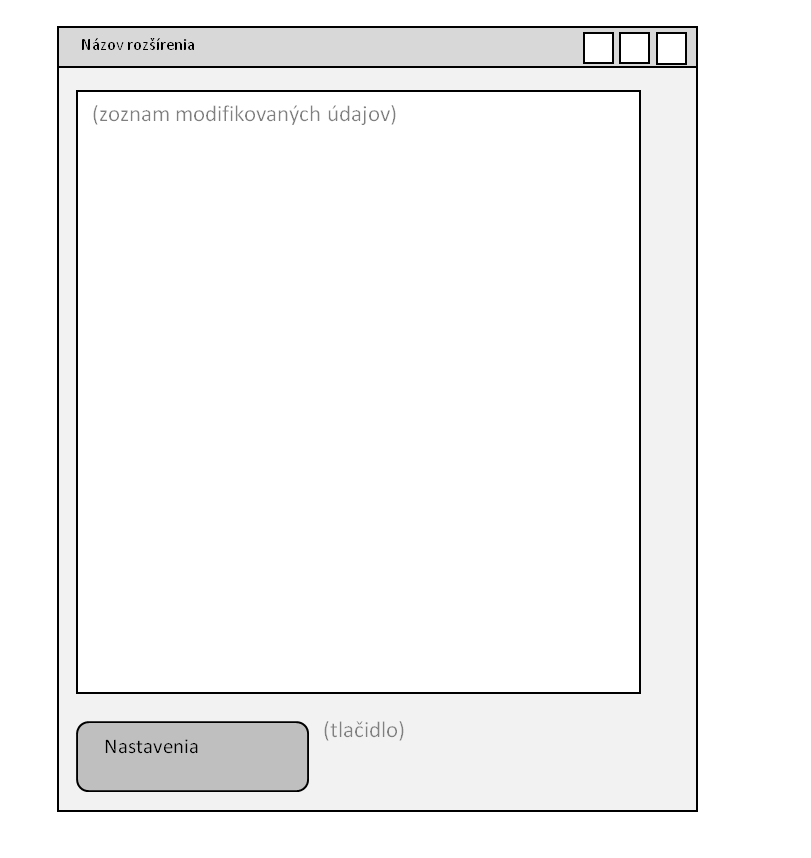
\includegraphics[width=8cm]{img/vzhlad.png}
  \caption{Predpokladan??? vzh???ad roz??????renia.}
  \label{vzhladobr}
\end{figure}	 
\noindent D???le???itou po???iadavkou kladenou na roz??????renie bolo pr???jemn??? pou??????vate???sk??? rozhranie.\cite{anonlib} Z~tohto d???vodu malo roz??????renie obsahova??? zoznam modifikovan???ch vlastnost??? a tla???idlo pre pr???stup k nastaveniam roz??????renia v jednoduchej a praktickej forme. Predpokladan??? vzh???ad je zobrazen??? na obr???zku ???. \ref{vzhladobr}.

\begin{algorithm}
\lstset{
    language=C,
    basicstyle=\small\sffamily,
    frame=none,
    numbers=left,
    xleftmargin=5.0ex,
    numberstyle=\tiny,
    stepnumber=1,
    showstringspaces=false,
    keywordstyle=\color{blue}\bfseries
    }
\lstset{emph={%  Adjust any special keywords
    printf%
    },emphstyle={\color[rgb]{1,0,0}\bfseries}%
}%
\begin{lstlisting}
/* Hello World program */

#include<stdio.h>

struct cpu_info {
    long unsigned utime, ntime, stime, itime;
    long unsigned iowtime, irqtime, sirqtime;
};

main()
{
    printf("Hello World");
}\end{lstlisting}
 \caption{Uk???ka algoritmu}
 \label{euclid}
\end{algorithm}